\chapter{Calculus I: Limits, Continuity and Derivative}
\begin{quote}
    Calculus, the mathematics of change, and change, mysterious. Some things grow imperceptibly... others zoom... hair grows slowly and suddenly cut... temperatures rise and fall... smoke curls through the air... planets wheel through space... and time, time never stops... - Cartoon Guide to Calculus
\end{quote}
Imagine you're sitting in a car with your family, driving along a winding mountain road. The scenery outside is breathtaking, with lush green forests, towering cliffs, and a deep blue sky. As you cruise along, you can't help but notice how the world around you is constantly transforming.\\
Now, let's say you're curious about how fast things are changing. You're particularly interested in how quickly your car is ascending the mountain. You pull out your trusty stopwatch and start measuring the time it takes to climb each mile of the road. You also jot down your car's speed at each mile marker.\\
As you collect this data, something remarkable happens. You realize that the speed of your car is not constant—it varies with each mile. Sometimes you're going uphill at a slow pace, and other times you're speeding down a hill, faster than you thought possible.\\
What's even more intriguing is that you notice a pattern: the steeper the incline, the slower your car seems to go. Conversely, when the road levels out or slopes downward, your car speeds up. This variation in speed as you move along the road is what we call...\\
\section{The Rate of Change}
In a still shot of a baseball game, the ball is clear, not moving at the instant of the photo. A good camera can take many such photos each with the ball clear and stopped.\\ \begin{figure} [h]
    \centering
    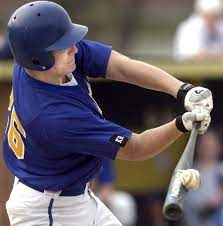
\includegraphics[width=0.5\linewidth]{Photos/Baseball calc.png}
    \caption{Is the ball moving? How do you know?\\
    courtesy, Champaign News-Gazette and photographer Robin Scholtz, 2003}    
\end{figure}
So if in any instant the ball is stopped, how is it truly moving? This is known as Zeno's paradox. The answer is rather simple. The ball, like every other moving object, has an unseen invisible quantity called velocity which is dictating its speed and direction.\\
While we can define velocity as rate of change of distance(displacement is more physically accurate as it also encompasses the direction), what about changing velocity?\\
As a baseball is thrown in the air, its velocity decreases as it slows down before it stops at its highest point. It then comes down, speeding up along the way.\\
However, here is a small issue. The speedometer of the car was showing you a speed all the time without ever actually having memory of what time it is and how much distance we had travelled.\\ 
How did that work? The speedometer was showing us the speed in the last 0.01 sec or even smaller. That was the cars instantaneous speed.\\
If this feels sort of strange, it should. This is all kind of paradoxical, as we are trying to look for the speed of something in a snapshot, which is not possible as we cannot divide by zero.\\
\begin{figure} [h]
    \centering
    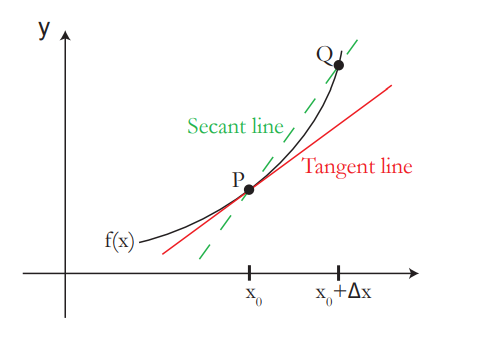
\includegraphics[width=0.5\linewidth]{Photos/Calculus tangent.png}
    \caption{The graph at heart of calculus}
    
\end{figure}
If the $f(x)$ is out distance function and time is along the $x$ axis, we can represent velocity between time $x_0$ and $x_0+\Delta x$ as the slope of the line between $f(x_0)=P$ and $f(x_0+\Delta x)=Q$.\\
As $\Delta x \rightarrow 0$, $f(x_0+\Delta x)=Q \rightarrow P$, which makes the secant between $P$ and $Q$ a tangent at $P$ of which we can find the slope off.\\
This is essentially what your speedometer does, it measures the slope of the the tangent of your distance graph.\\
This is essentially what calculus is all about.\\
\section{Some functions}
We will end up using some functions again and again in calculus. These functions using in combination with each other make up most of the things we see in physics, which is the major use of calculus. I will take this moment to remind you that a function is a relation from a domain to co-domain.\\
\subsection{Constant Function}
A simple function which returns the same value even in plugging out different values. Domain is  $x \in \mathbb{R}$, while the co-domain is a single Real number. \\
\begin{figure} [h]
    \centering
    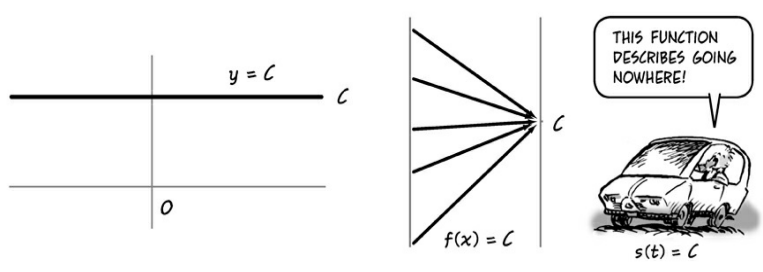
\includegraphics[width=0.5\linewidth]{Photos/Constant function.png}
    \caption{The constant function}
    
\end{figure}
\subsection{Power Function}
These are the functions with formulas $x, x^2, x^3, \dots x^n$, where $n$ is a positive integer. When n is even, these functions all have bowl-shaped graphs as $(-x)^{2n} = x^{2n}$.\\ If n is odd, then $(-x)^{2n-1} = -(x^{2n-1})$, causing the graphs bend downward on the left.
\begin{figure} [h]
    \centering
    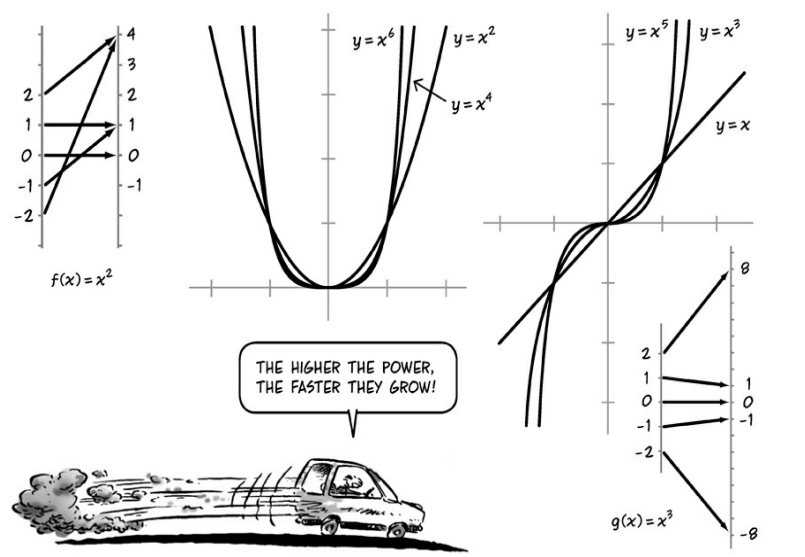
\includegraphics[width=0.5\linewidth]{Photos/Power Function.png}
    \caption{Power Function}
    
\end{figure}
\subsection{Polynomials}
Polynomials are basically made by multiplying powers by constants and adding them. You already know from algebra that a polynomial with degree $n$ has at most $n$ roots or $n$ points where the graph cuts zero. We can also notice that every polynomial either goes to $\infty$ or $-\infty$, so every time it cuts at zero more than once, it will also have a turning. So basically,  it has at most $n-1$ turnings. The turnings will become use full in a minute.
\subsection{Negative powers}
We can also write negative powers using the fact $x^{-n}=\frac{1}{x^n}$. Their graph also varies according to the parity of $n$.\\
\begin{figure} [h]
    \centering
    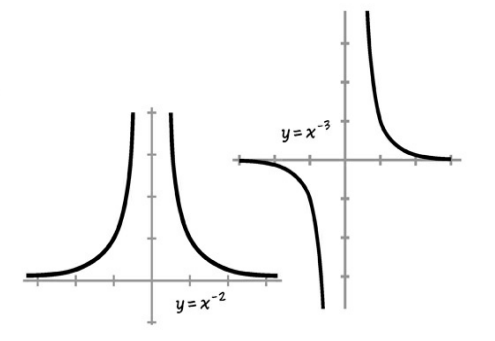
\includegraphics[width=0.5\linewidth]{Photos/Negative powers.png}
    \caption{Negative Powers}
    
\end{figure}
\subsection{Fractional Powers}
We can also plot $x^{\frac{1}{n}}=\sqrt[n]{x}$. Also without any surprise, you might have already understood that it also depends on pairity.\\
\begin{figure} [h]
    \centering
    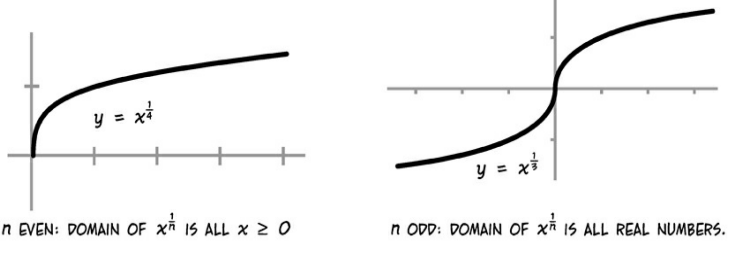
\includegraphics[width=0.5\linewidth]{Photos/Fractional Powers.png}
    \caption{Fractional Powers}
    
\end{figure}
\subsection{Exponential functions}
Power functions: We get large pretty quickly\\
Exponential functions: Hold my cup...\\
Exponential functions are defined as $f(x)=a^x$ where $a$ is constant.  Physicists like using $e$ as the base where $e$ is Euler's number and is equal to $2.718 \dots$\\
Like $\pi$ it is irrational, however unlike $\pi$, it's definition is not geometric.  It was arrived upon by Jacob Bernoulli while pondering the given question\\
\begin{example}
    An account starts with $1$ dollar and pays $100$ percent interest per year. If the interest is credited once, at the end of the year, the value of the account at year-end will be $2$ dollars. What happens if the interest is computed and credited more frequently during the year?
\end{example}
Using our knowledge of sequence and series, we could compute that if the interest was compounded $n$ times an year, we would get $(1+\frac{1}{n})^n$.  If we keep making $n$ larger and larger, till it approaches $\infty$, we'll be left with $e$. How exactly? We'll talk about that in just a minute \\
We can using algebra also say that $e^r=a$ will have an unique solution for $r$ as long as $a \neq 0$. This is used so often that we have a notation for it: $\ln(a)=r$ where $\ln$ refers to the natural logarithm. It's properties are discussed in greater detail in the logarithm's chapter. However, using only the fact that it exists we can say $f(x)=e^{rx}$. \\
This graph grows exponentially for $r>0$, is constent for $r=0$ and decays exponentially for $r<0$.\\
\subsection{Trigonometric Functions}
If you are unfamiliar with trigonometry, I recommend reading through that chapter before continuing this .\\
\begin{figure} [h]
    \centering
    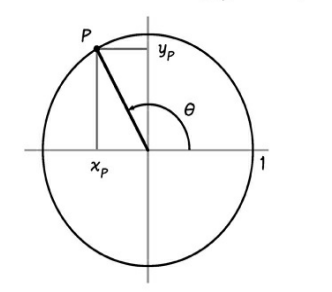
\includegraphics[width=0.5\linewidth]{Photos/Trigonometric circle.png}
    \caption{Meet the unit circle}
    
\end{figure}
Here we have a circle of radius $1$ and make two perpendicular lines through the center. A radii is made which goes from the center to some point on the circumference $P$ making an angle $\theta$  with the horizontal, which is measured in radians. Radians are another way to measure angles which is the norm in physics. It basically is the arc length of the arc subtended by your angle divided by the radius.  Physicist's like it better as it doesn't use an abstract number 360 as the reference for the angles instead uses an physical quantity\\
But back to the diagram, The perpendicular distance of this from the $y$ axis is called $\cos\theta$ and the perpendicular distance from the $x$ axis is called $\sin(\theta)$ . We define $\tan(\theta) =\frac{\sin(\theta)}{\cos(\theta)}$\\
A trigonometric function refers to $f(x)=\sin(x);f(x)=\cos(x); f(x)=\tan(x)$ or  a combination of them with coefficients  where the domain is $x \in \mathbb{R}$ and the co-domain for $\sin(x)$ and $\cos(x)$ is $\{-1,1\}$. The co-domain is all real numbers for $\tan(x)$. \\
\begin{figure} [h]
    \centering
    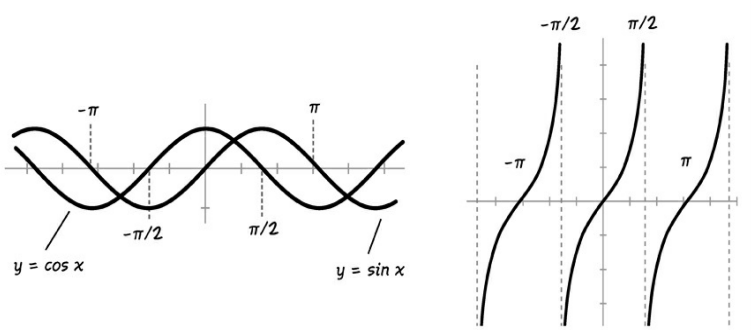
\includegraphics[width=0.5\linewidth]{Photos/Trigonometric functions.png}
    \caption{Trigonometric Functions}
    
\end{figure}
\subsection{Composing Functions}
A composing function is defined as $f(x)=h(g(x))$ basically, a combination of two functions. NOTE: While sometimes, $h(g(x))=g(h(x))$ this is often untrue. We should not interchange the functions unless we are absolutely sure we can.\\
\subsection{Inverting Functions}
If composing function $f(x)=h(g(x))=C$ where C is a constant then $h(x)$ is the inverse of $g(x)$ and vice versa. The inverse of a function $k(x)$ is sometimes denoted as $k^{-1}(x)$.
You may feel that an inverse composition may be switched around but consider this: $g(x)=x^2, h(x)=\sqrt{x}$ then while $f(x)=g(h(x))$ has a domain of all positive real numbers, $f(x)=h(g(x))$ has a domain of all real numbers; making them fundamentally different.\\
\section{Inverse Trigonometric functions}
This difference is even more profound with trigonometric functions(whose inverse are written as $\sin^{-1},\cos^{-1},\tan^{-1}$ and have domains of $(-1,1); (-1,1); \theta \in \mathbb{R}$ respectively.)\\
We need to note that while $\sin(x)$ keeps on going up and down, it is strictly increasing in the range $\frac{-\pi}{2}\leq x \leq \frac{\pi}{2}$. Fun fact: A lot of people refer to $\sin^{-1}$ as $\arcsin$. This is because it basically corresponds to the length of the arc the radii is subtending given the perpendiculer distence from the vertical.\\
\begin{figure} [h]
    \centering
    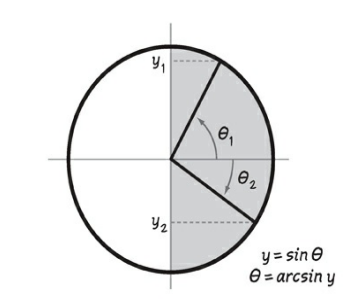
\includegraphics[width=0.5\linewidth]{Photos/Arcsin unit circle.png}
    \caption{The return of the unit circle}
\end{figure}
I expect you to find the co-domain of $\arccos$ by yourself now.
\begin{example}
    Find the co-domain of $\arccos$
\end{example}
Let's talk about $\arctan$. The co-domain of this is pleasantly surprising as it has a massive domain.\\
\begin{figure} [h]
    \centering
    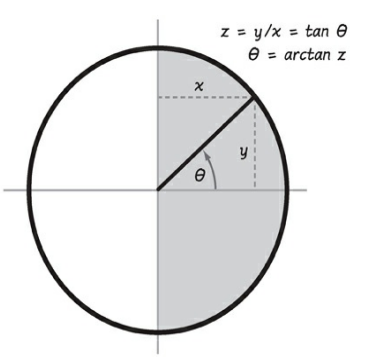
\includegraphics[width=0.5\linewidth]{Photos/Arc tan Unit Circle.png}
    \caption{The Unit Circle Awakens}
    
\end{figure}
\section{Derivative}
As derivative is the slope of a function $f(x)$ at a particular point, we can also plot the derivative as a function $f'(x)$ as we move that particular point.\\
\begin{theorem}
[Differentiation formula]
    \[f'(x)=\frac{f(x+h)-f(x)}{h}, h \rightarrow 0\] 
\end{theorem}
This is just formalization of the definition of derivative.\\
Using this definition, we can quite easily figure some more things.\\
\begin{theorem}
[Two truths of differentiation]
    $(f(x)+g(x))'=f'(x)+g'(x)\\
    \therefore (Cf(x))'=Cf'(x)$ where $C$ is a constant
\end{theorem}
While this seems both trivial and extraordinary, here is the proof
\begin{proof}
    $(f(x)+g(x))'\\
    =\frac{f(x+h)+g(x+h)-f(x)-g(x)}{h}\\
    = \frac{f(x+h)-f(x)}{h}+\frac{g(x+h)-g(x)}{h}\\
    = f'(x)+g'(x)$
\end{proof}
We will also prove some standard derivatives which you should remember(just the identity, the proof is obvious).
\begin{theorem}
[Power rule of differentiation]
    If $f(x)=x^n$,\\
    $f'(x)=nx^{n-1}$
\end{theorem}
\begin{proof}
    $f'(x)=\frac{{x+h}^n-x^n}{h}\\
    = \frac{x^n+nx^{n-1}h+\dots+nxh^{n-1}+h^n -x^n}{h}
    = nx^{n-1}+\binom{n}{2}x^{n-2}h+\dots +nxh^{n-2}+h^{n-1} \text{Using } h \rightarrow 0\\
    =nx^{n-1}$
\end{proof}
With this much, we are now qualified enough to find the derivative of all polynomials.
\begin{theorem}
    If $f(x)=\sin(x)$, then:\\
    $f'(x)=\cos(x)$\\
    If $f(x)=\cos(x)$, then:\\
    $f'(x)=-\sin(x)$
\end{theorem}
\begin{proof}
    $f'(x)=\frac{\sin(x+h)-\sin(x)}{h} \text{By the trigonometric property for } \sin(\alpha+\beta)\\
    = \frac{\sin(x)\cos(h)+\cos(x)\sin(h)-\sin(x)}{h}\\
    = \cos(x)\frac{\sin(h)}{h}+\sin(x)\frac{\cos(h)-1}{h}$
    We can notice that $\sin(h)=h$ for small values of $h$ as the perpendicular distance to horizontal and the arc length are almost equal.\\
    We also need to notice that $\cos(h)-1$ is almost equal to $0$ as the perpendicular distance to vertical is almost equal to the radius of the unit circle which is $1$.\\
    $\therefore \cos(x)\frac{\sin(h)}{h}+\sin(x)\frac{\cos(h)-1}{h}\\
    = \cos(x)\frac{h}{h}+\sin(x)\frac{0}{h}
    = \cos(x)$
\end{proof}
I'll leave the full proof for the derivative of $\cos(x)$ to you but the simple, non trigonometric, proof without words is in noticing that $\cos(x)$ is exactly like $\sin(x)$ shifted left by $\frac{\pi}{2}$.\\
\begin{figure} [h]
    \centering
    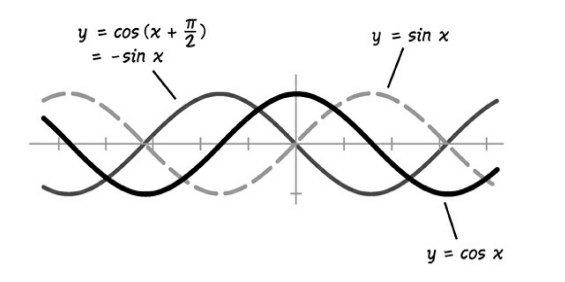
\includegraphics[width=0.5\linewidth]{Photos/Cos derivative proof without words.png}
    \caption{A proof without words}
    
\end{figure}
We'll come to $\tan(x)$ in a minute.
\begin{theorem}
    If $f(x)=e^x$:\\
    $f'(x)=e^x$\\
    $\therefore f(x)=a^x=f'(x) \iff a=e$.
\end{theorem}
This is what makes $e$ so special.
\begin{proof}
Let $f(x)=a^x=f'(x)$
    $f'(x)=\frac{a^{x+h}-a^x}{h}=a^x\\
    \iff a^x\frac{a^h-1}{h}=a^x\\
    \iff \frac{a^h-1}{h}=1\\
    \iff a^h=1+h$
    Remember the definition of $e$?, This is where that definition becomes significant(we'll prove it, wait for it). As $e=(1+\frac{1}{n})^n, n \rightarrow \infty$, we can set $h \rightarrow \frac{1}{n} \rightarrow 0$\\
    $\therefore e=(1+h)^{\frac{1}{h}}\\
    \therefore e^h=1+h$\\
    Which implies, $a=e$\\
    Hence proved.
\end{proof}
One of my most favorite proofs.
\section{Some more notation}
Calculus has had a dark history. Newton and Leibniz contested on who had invented it. The thing is that they both assumed that the other had copied it. Historical records show that the discovery was 1. independent, 2. already discovered approximately 2000 years ago by the Greek, Chinese, Arabic and Indian mathematicians 3. already in use in different forms by modern mathematicians and physicists like Galileo and Kepler\\
So in classic European fashion, they took something that was already there, gave it a name and then argued over who 'discovered' it.\\
What they did do was give us some sort of a better notation system. Till now we were using the Newton's notation where derivatives are shown as $f'(x)$ but we'll use Leibniz notation a bit more in the future as it simplifies a lot of things which Newton would complicate.\\
In Leibniz notation, the derivatve is taken of an equation rather than of a function. For example:\\
$y=x^2\\
\therefore \frac{dy}{dx}=2x$
Here, $\frac{dy}{dx}$ implies the derivative. The $d$ here is a version of $\Delta$, which is what we use to show big change, but $d$ shows microscopic changes. Basically, this is just the original meaning of differentiation.\\
We also need to notice that we just multiplied the entire equation by $\frac{d}{dx}$ and solved the derivatives and got the result.\\
This makes the two truths feel like an elementary fact.\\
\section{Product and Quotient rules}
\begin{theorem}
[Product rule]
    $(f(x)g(x))'=f'(x)g(x)+f(x)g'(x)$
\end{theorem}
\begin{proof}
We'll take $f(x+h)=f(x)+\Delta(f)$ where $h,\Delta(f) \rightarrow 0$\\
    $\therefore (f(x)g(x))'=\frac{f(x+h)*g(x+h)-f(x)g(x)}{h}\\
    = \frac{(f(x)+\Delta(f)*(g(x)+\Delta(g)-f(x)g(x)}{h}\\
    = \frac{f(x)g(x)+g(x)\Delta(f)+f(x)\Delta(g)+\Delta(f)\Delta(g)-f(x)g(x)}{h}\\
    = g(x)\frac{\Delta(f)}{h}+f(x)\frac{\Delta(g)}{h}+\frac{\Delta(f)\Delta(g)}{h}$\\
    Using the fact that $\Delta(f),\Delta(g) \rightarrow 0$ and $f(x+h)-f(x)=\Delta(f)$ and $g(x+h)-g(x)=\Delta(g)$\\
    $g(x)\frac{\Delta(f)}{h}+f(x)\frac{\Delta(g)}{h}+\frac{\Delta(f)\Delta(g)}{h}\\
    = g(x)\frac{f(x+h)-f(x)}{h}+f(x)\frac{g(x+h)-g(X)}{h}\\
    =g(x)f'(x)+g'(x)f(x)$
\end{proof}
Also I'd like you to note that, by the same proof, if we want to differentiate more than two functions we can go for: $(fgh\dots)'=f'gh\dots+fg'h\dots+fgh'\dots$\\
\begin{theorem}
[Reciprocal rule]
    $(\frac{1}{f(x)})'=\frac{-f'(x)}{(f(x))^2}$
\end{theorem}
\begin{proof}
    $(\frac{1}{f(x)})'=\frac{\frac{1}{f(x+h)}-\frac{1}{f(x)}}{h}\\
    =\frac{\frac{f(x)-f(x+h)}{f(x+h)f(x)}}{h}\\
    =\frac{-f'(x)}{f(x+h)(f(x)} \text{Using } h \rightarrow 0\\
    =\frac{-f'(x)}{(f(x))^2}$
\end{proof}
Combining the product and reciprocal rule gives us:\\
\begin{theorem}
    [Quotient Rule]
    $(\frac{f(x)}{g(x)})'=\frac{f'(x)g(x)-f(x)g'(x)}{(g(x))^2}$
\end{theorem}
We are now powerful enough to solve a few more differential questions:\\
\begin{example}
    For $f(x)=\tan(x)$, compute:\\
    $f'(x)$
\end{example}
\begin{proof}
    [Solution]
    We know that the formula for $\tan{\alpha+\beta}$ is quite messy. However, we are also know that $\tan(\theta) = \frac{\sin(\theta)}{\cos(\theta)}$ as well as the derivatives for $\sin(\theta)$ and $\cos(\theta)$, this seems like an use the quotient rule.\\
    $\therefore f'(x)=\frac{(\sin(x))'\cos(x)-(\cos(x))'\sin(x)}{\cos^2(x)}\\
    =\frac{\cos^2(x)+\sin^2(x)}{\cos^2(x)}$\\
    We know that $\sin^2(x)+\cos^2(x)=1$ using the unit circle,\\
    $\therefore \frac{\cos^2(x)+\sin^2(x)}{\cos^2(x)}\\
    = \frac{1}{\cos^2(x)}\\
    = \sec^2(x)$\\
    The final step is by the definition that $\frac{1}{\sin}=\csc; \frac{1}{\cos}=\sec; \frac{1}{\tan}=\cot$
\end{proof}
I will leave it to you as exercise to differentiate the rest of the trigonometric functions by yourself.\\
\begin{theorem}
    $x^{-n}=-nx^(-(n+1))$
\end{theorem}
While, this is exactly what the power rule states. It's proof is different from that of the power rule as we can't use the binomial expansion here. However, it's trivial as we are just using the reciprocal rule and the power rule together. I expect that you'll take it upon yourself to prove it once for practice.
\section{Chain rule}
While we can differentiate a lot of things, we still fail to differentiate things like $e^{2x}$ or $\sin(\cos(x))$.\\
Here is where the chain rule comes.\\
\begin{theorem}
    $f(g(x))'=g'(x)f'(g(x))$
\end{theorem}
This probably looks worse than it actually is. It's proof will appear in a minute. But till then let's do a question to understand this better.\\
\begin{example}
    $\frac{d}{dx} e^{2x}$
\end{example}
\begin{proof}
    [Solution]
    The chain rule basically states that for the derivative of $f(g(x))$ we will first take $f'(x)$ and plug $g(x)$ in place of $x$. We'll then multiply that by $g'(x)$\\
    In this case, $f(x)=e^x \implies f'(x)=e^x$ and $g(x)=2x \implies g'(x)=2$, therefore:\\
    $(e^{2x})'=2e^{2x}$
\end{proof}
\begin{example}
    $\frac{d}{d\theta}\sin(\cos(\theta))$
\end{example}
I believe this one will be a cake walk for you to do.\\
Now let's talk about inverses. The chain rule can solve for the inverse given we know the derivative of the original function.\\
\begin{theorem}
    [Inverse Rule]
    $(f^{-1}(x))'=\frac{1}{f'(f^{-1}(x)}$
\end{theorem}
\begin{proof}
    $x=f(f^{-1}(x))\\
    \iff \frac{dx}{dx}=\frac{d}{dx}f(f^{-1}(x))\\
    \iff 1=f{'}^{-1}(x) \cdot f'(f^{-1}(x))\\
    \iff (f^{-1})'(x)=\frac{1}{f'(f^{-1}(x)}$
\end{proof}
If you use this formula on $x^{\frac{1}{n}}$, you'll get what we get by the power rule. If you think that's cool, hold my cup:\\
\begin{theorem}
    $\frac{d}{dx} \ln(x)=\frac{1}{x}$
\end{theorem}
This looks wild. How did this even happen?\\
\begin{proof}
    As $f(x)=\ln(x)$ is the inverse of $g(x)=e^x \implies g'(x)=e^x$ , we can use the inverse rule.\\
    $\frac{d}{dx} \ln(x) = \frac{1}{e^{\ln(x)}}=\frac{1}{x}$
\end{proof}
This obviously doesn't happen with other functio...\\
\begin{theorem}
    $\frac{d}{dx} \arcsin(x)=\frac{1}{\sqrt{1-x^2}}$
\end{theorem}
\begin{proof}
    As $f(x)=\arcsin(x)$ is the inverse of $g(x)=\sin(x) \implies g'(x)=\cos(x)$ , we can use the inverse rule.\\
    $\frac{d}{dx} \arcsin(x) = \frac{1}{\cos(\arcsin(x)}$\\
    As $\sin^2(x)+\cos^2(x)=1$, therefore $\cos(x)=\sqrt{1-\sin^2(x)}=\sqrt{1-x^2}$\\
    Plugging in $x=\arcsin(x)$ we get: $\cos(x)=\sqrt{1-x^2}$, therefore:\\
    $\frac{1}{\cos(\arcsin(x)} = \frac{1}{\sqrt{1-x^2}}$
\end{proof}
So maybe this the only trig funct...\\
\begin{theorem}
    $\frac{d}{dx} \arctan(x)=\frac{1}{1+x^2}$
\end{theorem}
\begin{proof}
    As $f(x)=\arctan(x)$ is the inverse of $g(x)=\tan(x) \implies g'(x)=\sec^2(x)$ , we can use the inverse rule.\\
    $\frac{d}{dx} \arctan(x) = \frac{1}{\sec^2(\arctan(x)}$\\
    As $\sec^2(x)-\tan^2(x)=1$(Just write both in terms of $\sin$ and $\cos$ and it will become obvious), therefore $\sec^2(x)=\tan^2(x)+1$\\
    Plugging in $x=\arctan(x)$ we get: $\sec^2(\arctan(x))=\tan^2(\arctan(x))+1=x^2+1$, therefore:\\
    $\frac{1}{\sec^2(\arctan(x)} = \frac{1}{1+x^2}$
\end{proof}
Also, as you might have already guessed. The same happens to every trigonometric function. I leave the proof up to you.\\
The strange part is that nobody has an intuitive explanation why this happens. It just does through proven formulas and we don't question it.\\
But wait, we haven't proven the chain rule. So let's do it.\\
Let's go on a small tangent first. Remember that functions are just arrows from the domain to co-domain?\\
So we can write functions in a parallel view like this.
\begin{figure} [h]
    \centering
    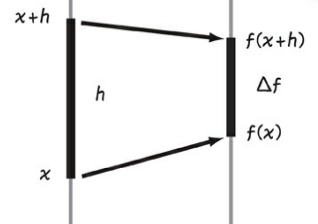
\includegraphics[width=0.5\linewidth]{Photos/Parallel view of function_ Chain rule.png}
    \caption{Parallel view of function}
    
\end{figure}
Here I ask you a simple question, by what scale has $h$ been increased due to the function? $\frac{\Delta f}{h}$ is the obvious answer.\\
But what happens when $h \rightarrow 0$, things start to breakdown as they get smaller, don't they?\\
Let's talk about what we mean to be small. Smallness is relative, a mouse is small in comparison to an elephant. A flea is small in comparison to the mouse. The flea is beneath notice in comparison to the elephant.\\
In terms of math, elephant refers to macro numbers like $x, f(x)$ while they can be zero in some cases, they are mostly not.\\
The increment $h$ is the mouse. Which while very small, is not beyond notice. However, anything which when divided by $h$ is approaches zero can be considered a flea. This makes $h^2, h^3, h^{\frac{4}{3}}$ fleas as $h \rightarrow 0$.\\
We can say that $\frac{\text{flea}}{h}=\text{mouse}$ (as it is approaching 0, not reaching it)\\
We can also say that $h*\text{mouse}=\text{flea}$\\
This all may seem interesting but where are we going with this?\\
Remember the secant and tangent which we used to create the differentiation formula? We are finally going to return to it.\\
We know that $\frac{\Delta f}{h}=f'(x)$ as $h \rightarrow 0$\\
Then we can say $\frac{\Delta f}{h}-f'(x)=0$ as $h \rightarrow 0$\\
But as $h$ approaches $0$, not reaches it,  $\frac{\Delta f}{h}-f'(x)= \text{mouse}$\\
Multiplying by $h$ gives us: $\Delta f = hf'(x)+ \text{flea}$\\
Graphically this is nothing but the fact that as $P$ and $Q$ come closer, the secant and tangent have the difference of the most minuscule flea.\\
This in terms of our parallel view of functions we can now say that the scaling factor was $f'(x)h+\text{flea}$ where the flea can be ignored. This is monumental as we only need the value of $x$ to actually find by what the function becomes.\\
This proves the chain rule almost instantly.\\
\begin{proof}
    \begin{figure} [h]
    \centering
    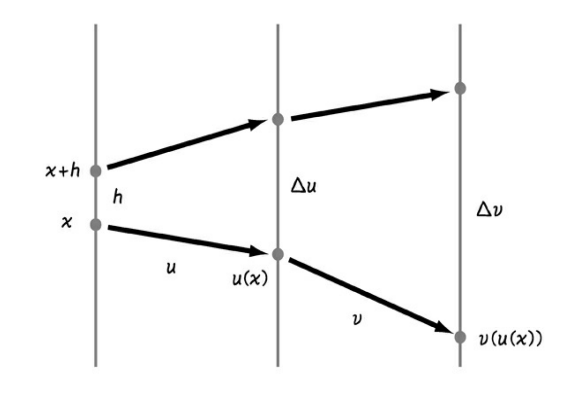
\includegraphics[width=0.5\linewidth]{Photos/Chain rule proof.png}
    \caption{The chain rule, in parallel form}
\end{figure}
We can say that $\Delta u= u'(x)h$ and therefore:\\
$\Delta v= v'(u(x))\Delta u\\
=v'(u(x))u'(x)h\\
\therefore v(u(x))'=\frac{\Delta v}{h}=v'(u(x))u'(x)h$\\
And we are done.\\
\end{proof}
While all this is sure neat, but what is it actually used for? You'll see it in a minute.\\
\section{Limits}
All this time we have been taking derivatives of functions assuming that they exist. What about when they don't? What about times where a point is not in the domain of $f(x)$ but is in the domain of $f'(x)$? What about all that?\\
Imagine a blind pirate captain named Goldeyes who lands on an island with a mysterious heavy object hidden in a hole. He faces a dilemma: should he try to retrieve this object for his ship's treasure or leave it behind? To help him decide, Goldeyes turns to his two most trusted companions for their opinions. Here are the three possible outcomes:\\
Disagreement: Both companions provide conflicting opinions—one claims it's just a common rock, while the other insists it's the valuable treasure of John Timbers. In this scenario, Goldeyes is left uncertain about the true nature of the object. Consequently, he decides to leave it on the island, as he cannot confidently determine its identity.\\
Partial Information: One of his companions confidently identifies the object as John Timbers' treasure, but the other companion is unsure and cannot confirm. Again, Goldeyes is faced with uncertainty, and he opts to leave the object behind because he lacks a clear understanding of what it truly is.\\
Consensus: In the final case, both companions unanimously agree that the object is the same, whether they both claim it's a rock or John Timbers' gold. Goldeyes, despite being blind and unable to verify the object himself, trusts the consensus of his companions and takes action accordingly. If they both say it's gold, he will take it as treasure(even if it is rock); if they both say it's a rock, he will disregard it as a worthless item(even if it is tresure).\\
How does this have anything to do with calculus? In a minute it will become clear.\\
Till now we were dealing with continuous functions. A continuous graph refers to functions whose graph can be drawn without lifting the pen. However, we need to understand that some graphs are discontinuous at a number of points.\\
Let's consider the function $f(x)=\frac{x^2-9}{x-3}$ which has a domain of $\mathbb{R}-3$ as $\frac{0}{0}$ is undefined. This also makes it discontinuous as the graph has a hole at $x=3$\\
However, for rest of the real numbers, $f(x)=x+3$. So if we look slightly on the left of $x=3$ we can get a number close to $6$ and just on the right of $x=3$ we have a number close to $6$ as well. So we can say that: $\lim_{x \to 3} \frac{x^2-9}{x-3}=6$. We need to understand that like Captain Goldeye's we still have zero idea on what is in the hole, but based on what two people are telling us we are making out mind on what is in the hole. This is called limit of a function $f(x)$ for $x=a$.\\
The limit for $f(x)$ at $x=\alpha$ is said to exist if and only if $\lim_{x \to \alpha^-} f(x)=\lim_{x \to \alpha^+} f(x)$ and then $\lim_{x \to \alpha^-} f(x)=\lim_{x \to \alpha^+} f(x)=\lim_{x \to \alpha} f(x)$\\
However, this rule has an exception. If both the left hand limit(LHL) and the right hand limit(RHL) are going to $\infty$ or $-\infty$ the limit is known as infinite limit. This limit doesn't exist as infinite is very large. Let me explain.\\
For example, if a man from Paris and a woman from Bordeaux leave for Russia, do they meet? Unless they are characters in a rom-com, the event seem unlikely as Russia is quite large.\\
The same happens here. Infinity is quite large, how do we know that both the LHL and RHL meet?\\
\begin{theorem}
[Fundamental theorem of Limits]
    If $\lim_{x \to \alpha}f(x)=l$ and $\lim_{x \to \alpha}g(x)=k$ then:\\
    $\lim_{x \to \alpha}f(x) \pm g(x)=l \pm m\\
    \lim_{x \to \alpha}f(x) \cdot g(x)=l \cdot m\\
    \lim_{x \to \alpha}\frac{f(x)}{g(x)}=\frac{l}{m}\\
    \lim_{x \to \alpha}nf(x)=n\lim_{x \to \alpha}f(x)=nl\\
    \lim_{x \to \alpha}g(f(x))=g(\lim_{x \to \alpha}f(x))=g(l)$ provided $g$ is continuous at $g(x)=m$
\end{theorem}
We can now do some simple questions pertaining to limits.\\
\begin{example}
    Let $f(x) =
\begin{cases}
    \frac{1}{2} & \text{for } x > 1 \\
    0 & \text{for } x = 1 \\
    \frac{1}{2} & \text{for } x < 1
\end{cases}$\\
What is $\lim_{x \to 1} f(x)$?
\end{example}
I recommend you to think about this question and make a prediction about this answer. Do not look at the solution. Done.\\
\\
The answer is not $0$. Notice that the function is discontinous at $x=1$. We have a hole in the graph and what did Captain Goldeyes teach us? We will trust the LHL and RHL even if what they say is untrue. Here slightly less than $1$ would give us $\frac{1}{2}$ and so would slightly greater than $1$. Hence, the limit is $\frac{1}{2}$.\\
It is only in continuous functions(or continuous regions of discontinuous functions) where we can plug in whatever the number is approaching to and expect the limit to be the same. For a point of discontinuity, we will look at the LHL and RHL.\\
While the above examples was 150\% unnecessary and just me trying to be a little tricky and cheeky as this limit has no real significance, we should ask where limits are used?\\
In certain time functions which occur in physics, the discontinuous points lead to indeterminate forms. These are seven things which are indeterminable in math. However, time is continuous so we are certain that the function needs to have a value. This is what limits allows us to do. The indeterminate forms are $\frac{0}{0}, \frac{\infty}{\infty}, 0 \times \infty, \infty - \infty, \infty^0, 0^0, 1^{\infty}$. Through algebraic manipulations, all these forms may be inter-converted.\\
Here are also some forms which a lot of people mistake for indeterminate but are actually not: $\infty+\infty=\infty, \infty \times \infty = \infty, \frac{\alpha}{\infty}=0$ if $\alpha$ is finite.\\ 
Also before someone tries to argue $\infty+\infty=\infty \iff 2=1$ remember, $\frac{\infty}{\infty}$ is indeterminate.\\
Also note: $\frac{\infty}{a}, \frac{a}{0}$ are also indeterminate for $\alpha \in \mathbb{R}$. They are not part of the seven forms as they have a variable as part of their formulation.\\
\begin{example}
    We know that for $\lim_{x \to 0}\frac{x^2}{x}$ no limit exists, as LHL $\neq$ RHL. Does $\lim_{x \to 0}\frac{\lfloor x^2 \rfloor}{x}$ exist(here $\lfloor a \rfloor$ refers to the greatest integer less than or equal to $a$?
\end{example}
Again I encourage you to think about this. Before we see the solution. While this is also like the previous is 150\% unnecessary and just me trying to be a little tricky and cheeky, it touches on some critical concepts.\\
\\
If you answered that the limit doesn't exist, you are wrong. The greatest integer function(GIF) causes a subtle but monumental change. Let's consider the LHL for maybe $x=-0.001$, $\frac{\lfloor {-0.001}^2 \rfloor}{-0.001}=\frac{\lfloor 0.000001 \rfloor}{-0.001}=\frac{0}{-0.001}=0$. If we do the same for RHL we can notice that the GIF has caused LHL $=$ RHL $=0$ and hence the limit is equal to $0$.\\
We can resolve indeterminacy in a few ways. We can Simplify, factorize or rationalize the function like we did with $f(x)=\frac{x^2-9}{x-3}$. We can use certain standard limits which we will learn about in a moment. Or we can make some approximations and solve it, like we did with $f(x)=\frac{\sin(x)}{x}$. The most intuitive and simple one is using approximations. You'll see it destroy questions other methods took time around. The only thing is that you'll have to hold your curiosity as their proof is not gonna appear for quite some time, it is in another chapter. But for now, you'll have to trust me. If you do, then here are some common approximations:\\
\begin{theorem}
[Taylor-Maclaurin Series]
    $e^x=1+\frac{x}{1!}+\frac{x^2}{2!}+\frac{x^3}{3!}+ \dots$ \\
    $a^x=1+\frac{x\ln(a)}{1!}+\frac{x^2\ln^2(a)}{2!}+\frac{x^3\ln^3(a)}{3!}+\dots$
    $\ln(1+x)=x-\frac{x^2}{2}+\frac{x^3}{3}-\dots$ for $-1 < x \leq 1$\\
    $\sin(x)=x-\frac{x^3}{3!}+\frac{x^5}{5!}-\dots$\\
    $\cos(x)=1-\frac{x^2}{2!}+\frac{x^4}{4!}-\dots$\\
    $\tan(x)=x+\frac{x^3}{3}+\frac{2x^5}{15}+\dots$\\
    In general, $f(x)=f(0)+\frac{xf'(0)}{1!}+\frac{x^2f''(0)}{2!}+\frac{x^3f'''(0)}{3!}+\dots$
\end{theorem}
As a even further cheat, we normally use less than the first three terms in the approximations if $x \to 0$, mostly a single term does the trick. I call this the Brahmastra over the mythological weapon in Indian mythology which can destroy anything and everything the universe.\\
Let's explore the concepts more through some problems.\\
\begin{example}
    \[\lim_{x \to 3} \frac{x^2-2x-3}{x^2-4x+3}\]
\end{example}
\begin{proof}
    [Solution]
    $\frac{x^2-2x-3}{x^2-4x+3}\\
    = \frac{(x-3)(x+1)}{(x-3)(x-1)}\\
    =\frac{x+1}{x-1}\\
    \therefore lim_{x \to 3} \frac{x^2-2x-3}{x^2-4x+3}
    = lim_{x \to 3} \frac{3+1}{3-1}$ as the new function is continuous at $x=3$\\
    $= \frac{4}{2}=2$
\end{proof}
\begin{example}
    \[\lim_{x \to 2+\sqrt{3}}\frac{x^4-7x^3+14x^2-7x+1}{x^2-4x+1}\]
\end{example}
\begin{proof}
    [Solution]
    $\frac{x^4-7x^3+14x^2-7x+1}{x^2-4x+1}
    = \frac{(x^2-3x+1)(x^2-4x+1)}{x^2-4x+1}\\
    = x^2-3x+1\\
    \therefore \lim_{x \to 2+\sqrt{3}}\frac{x^4-7x^3+14x^2-7x+1}{x^2-4x+1}\\
    = \lim_{x \to 2+\sqrt{3}} x^2-3x+1$ as $x^2-3x+1$ is continuous at $x=2+\sqrt{3}$, we can plug it in to get the answer as $2+\sqrt{3}$ \\
\end{proof}
So those two were quite standard. Let's do something more fun!
\begin{example}
    \[\lim_{x \to 1} \frac{3-\sqrt{8x+1}}{5-\sqrt{24x+1}}\]
\end{example}
\begin{proof}
    [Solution]
    We can solve this in two ways. While one is more tedious other is just chad. We'll do the tedious one first.\\
    To prevent the need to type the limit again and again, assume it's presence throughout the solve.\\
    $\frac{3-\sqrt{8x+1}}{5-\sqrt{24x+1}}\\
    = \frac{3-\sqrt{8x+1}}{5-\sqrt{24x+1}}\cdot\frac{3+\sqrt{8x+1}}{5+\sqrt{24x+1}}\cdot\frac{5+\sqrt{24x+1}}{3+\sqrt{8x+1}}$\\
    Notice that the last fraction doesn't have any indeterminacy, and is continuous and can hence be separated from the limit using the properties of limits. Therefore we can write it as:\\
    $\frac{5}{3} \cdot \frac{9-8x-1}{25-24x-1}\\
    = \frac{5}{3} \cdot \frac{8\cancel{(x-1)}}{24\cancel{(x-1)}}\\
    = \frac{5}{3}*\frac{1}{3}=\frac{5}{9}$\\
    Now let's do it using the chad method.\\
    We want to use approximations, hence we need the limit to be tending to 0. We'll substitute $x=1+t$ and $t \to 0$,\\
    $\lim_{t \to 0} \frac{3-\sqrt{9+8t}}{5-\sqrt{25+24t}}$\\ While doesn't seem anything too special, remember the binomial approximation from chapter-9? Assume the limit to be present from here onward\\
    $=\frac{3-3(1+\frac{8}{9}t)^{\frac{1}{2}}}{5-5(1+\frac{24}{25}t)^{\frac{1}{2}}}\\
    = \frac{3-3(1+\frac{4t}{9}}{5-5(1+\frac{12t}{25}}\\
    =\frac{3(\frac{4t}{9})}{5(\frac{12t}{25})}\\
    =\frac{3}{5}\cdot \frac{4}{9} \cdot \frac{25}{12}\\
    =\frac{5}{9}$
\end{proof}
You may have felt that the chad method wasn't really that good...
\begin{example}
    \[\lim_{x \to 1} \frac{x}{\sqrt{1+x}-\sqrt{1-x}}\]
\end{example}
\begin{proof}
    [Solution]
    Using binomial approximation, \\
    $\frac{x}{\sqrt{1+x}-\sqrt{1-x}}
    = \frac{x}{\cancel{1}+\frac{x}{2}-\cancel{1}+\frac{1}{x}}\\
    =\frac{2\cancel{x}}{\cancel{x}}\\
    =2$
\end{proof}
I leave trying out the rigorous method to you. Let's now try a problem where the rigorous method will become so complex that I don't think it will be worth the time or effort.\\
\begin{example}
    \[\lim_{x \to 2} \frac{3-\sqrt[3]{x^2+5x+13}}{4-\sqrt{x^2+3x+6}}\]
\end{example}
\begin{proof}
    Let $x=2+t$ and $t \to 0$,\\
    $\frac{3-\sqrt[3]{x^2+5x+13}}{4-\sqrt{x^2+3x+6}}\\
    = \frac{3-\sqrt[3]{(t+2)^2+5(t+2)+13}}{4-\sqrt{(t+2)^2+3(t+2)+6}}\\
    = \frac{3-\sqrt[3]{(t^2+4t+4+5t+10+13}}{4-\sqrt{(t^2+4t+4+3t+6+6}}\\
    = \frac{3-\sqrt[3]{(t^2+9t+27}}{4-\sqrt{(t^2+7t+16}}$\\
    Remember the entire mice and flea discussion? Can we neglect the fleas($t^2$) as after all $t \to 0$?\\
    $=\frac{3-\sqrt[3]{(9t+27}}{4-\sqrt{(7t+16}}\\
    = \frac{3-3(1+\frac{t}{3})^{\frac{1}{3}}}{4-4(1+\frac{7t}{16})^{\frac{1}{2}}}\\
    = \frac{3(1-1-\frac{t}{9})}{4(1-1-\frac{7t}{32}}\\
    =\frac{3}{4} \cdot \frac{t}{9} \cdot \frac{32}{7t}\\
    =\frac{8}{21}$
\end{proof}
We need to make a small note here. We cannot just neglect powers which don't exist. For example in $\lim_{x \to 0}\frac{(x^2+x+1)-(x+1)}{x}$ we cannot neglect $x^2$ in comparison to $x$ as the $x$ itself is getting canceled out. Remember, size is relative. We need someone in comparison to actually make a neglection.\\
Now let's talk about some standard limits and why people who try to memorize them are ignorant fools.\\
\begin{theorem}
[Standard results]
    \begin{enumerate}
    \item $\lim_{x \to 0}\frac{\sin(x)}{x}=\lim_{x \to 0}\frac{\tan(x)}{x}=1$
    \item $\lim_{x \to 0}\frac{\arcsin(x)}{x}=\lim_{x \to 0}\frac{\arctan(x)}{x}=1$
    \item $\lim_{x \to \infty}(1+\frac{1}{x})^x=\lim_{x \to 0}(1+x)^{\frac{1}{x}}=e$
    \item $\lim_{x \to \infty}(1+\frac{a}{x})^x=\lim_{x \to 0}(1+ax)^{\frac{1}{x}}=e^a$
    \item $\lim_{x \to 0} \frac{e^x-1}{x}=1$
    \item $\lim_{x \to 0} \frac{a^x-1}{x}=\ln(a)$ for $a>0$
    \item $\lim_{x \to 0} \frac{\ln(1+x)}{x}=1$
    \item $\lim_{x \to \alpha}\frac{x^n-\alpha^n}{x-\alpha}=n\alpha^{n-1}$
\end{enumerate}
\end{theorem}
\begin{proof}
    The first and second were explained earlier using unit circle. If someone want's they can use the Taylor series but that's overkill.\\
    The third one is a specific case($a=1$) of the fourth which we'll prove. Assuming limit to be wherever necessary,\\
    Let $\lim_{x \to 0}(1+ax)^{\frac{1}{x}}=y\\
    \iff \frac{1}{x} \ln(1+ax)=\ln(y)\\
    \iff \frac{ax}{x}= \ln(y)$ This is using the Brahmastra.\\
    $\iff \ln(y)=a\\
    \iff y=e^a$\\
    The infinity form is just obtained by taking $x=\frac{1}{n}$.\\
    The fifth is a mild embarrassment using Brahmastra, $\frac{e^x-1}{x}=\frac{x+1-1}{x}=\frac{x}{x}=1$\\
    The sixth limit will use the same methodology. $\frac{a^x-1}{x}=\frac{e^{x\ln(a)}-1}{x}=\frac{x\ln{a}+1-1}{x}=\ln(a)$\\
    The seventh limit just shouts Brahmastra,\\
    $\frac{\ln(1+x)}{x}=\frac{x}{x}=1$\\
    The eight limit will however have to wait a minute.
\end{proof}
Taking the logarithm of the limit(as we did for the forth one) is quite a common technique to deal with limits with variable exponents and I refer to it as Vayuastra, as a reference to the Indian mythological weapon which gives the user complete control of the sky and air.
And third and final weapon for attacking limits is L'Hopital's rule, which I call Agniastra as a refrence to, you guessed it, Indian mythology. As Agniastra gives the user immense fire power, so does L'Hopital.\\
  \begin{theorem}
      [L'Hopital's Rule]
      \[\lim_{x \to x_0} \frac{f(x)}{g(x)}= \lim_{x \to x_0} \frac{f'(x)}{g'(x)}\]
      If and only if, $f(x)$ and $g(x)$ are differentiable on all points other than $x_0$ with $g'(x_0)\neq0$ and $\frac{f(x)}{g(x)}$ is indeterminate which means $f(x)$ or $g(x)$ are both either $0$ or $\infty$ 
  \end{theorem}
  \begin{proof}
      We know that $\Delta f=hf'(x) \iff f(x+h)-f(x)=hf'(x) \iff f(x+h)=f(x)+hf'(x)$\\
      Now we'll compute the limit for $x \to x_0$ where $f(x_0)=g(x_0)=0$\\
      $\lim_{x \to x_0} \frac{f(x)}{g(x)}\\
      = \lim_{x \to x_0, h \to 0} \frac{f(x+h)}{g(x+h)}\\
      = \lim_{x \to x_0, h \to 0} \frac{hf'(x)+f(x_0)}{hg'(x)+g(x_0)}\\
      = \lim_{x \to x_0, h \to 0} \frac{\cancel{h}f'(x)}{\cancel{h}g'(x)}\\
      =\lim_{x \to x_0} \frac{f'(x)}{g'(x)}$\\
      Hence, proved.
  \end{proof}
This makes proving the eighth result a piece of cake.\\
$\frac{x^n-\alpha^n}{x-\alpha}=\frac{nx^{n-1}}{1}=nx^{n-1}$\\
All these standard results are hece quite easy to get and keeping them in the brain wastes the space which may be used elsewhere. Let's do some examples.\\
\begin{example}
    \[\lim_{x \to 0}\frac{3^x-1}{2^x-1}\]
\end{example}
\begin{proof}
[Solution]
    While this question is destroyed in shreds by Brahmastra, I'll use the Agniastra for instructive purposes.\\
    $(a^x)'=(e^{x\ln(a)})'$ we can use the chain rule here, to get:\\
    $=\ln(a)e^{x\ln(a)}\\
    = \ln(a)a^x$\\
    Using this in our limit gives:\\
    $\lim_{x \to 0}\frac{3^x-1}{2^x-1}\\
    = \lim_{x \to 0}\frac{\ln(3)3^x}{\ln(2)2^x}$ as the function is now continuous, we can just plug in $x=0$\\
    $=\frac{\ln(3)}{\ln(2)}
    =\log_2(3)$
\end{proof}
\begin{example}
    \[\lim_{x \to 0}\frac{1-\cos{3x}}{x^2}\]
\end{example}
\begin{proof}
    [Solution]
    For the first time, we'll have to use the Brahmastra upto two places.\\
    $\frac{1-\cos{3x}}{x^2}\\
    =\frac{1-(1-\frac{(3x)^2}{2!}}{x^2}\\
    =\frac{9\cancel{x^2}}{2\cancel{x^2}}\\
    =\frac{9}{2}$
\end{proof}
\section{Continuity}
As we have already defined, continuity refers to the fact a graph(or a region of it) can be drawn without lifting the pencil. However, more formally:\\
\begin{definition}
    A function $f(x)$ is continuous at $x=a$ if and only if:\\
    $f(a^-)=f(a^+)=f(a)$
\end{definition}
Basically the right hand function must agree with the left hand function as well as the instantaneous value. Unlike with limits, here $f(a)$ actually matters.\\
\begin{example}
    Let $f(x)=\begin{cases}
        (1+x)^{\frac{1}{x}} & \text{for } x > 0 \\
    a & \text{for } x = 0 \\
    \frac{1-\cos(x)}{bx^2} & \text{for } x < 0
    \end{cases}$\\
    If $f(x)$ is continuous at $x=0$, find $\lfloor a+b \rfloor$
\end{example}
\begin{proof}
    [Solution]
    Using the defination of continuity, we can say:\\
    $(1+x)^{\frac{1}{x}}=a=\frac{1-\cos(x)}{bx^2}$ for $x \to 0$\\
    You might recall that the limit of $(1+x)^{\frac{1}{x}}=e$ for $x \to 0$\\
    That means $a=e$. Let's now find $b$.\\
    $\lim_{x \to 0}\frac{1-\cos(x)}{bx^2}=e\\
    \iff \frac{1}{b} \lim_{x \to 0}\frac{1-\cos(x)}{x^2}=e\\
    \iff b=\frac{1}{e} \lim_{x \to 0}\frac{1-\cos(x)}{x^2}\\
    \iff b=\frac{1}{e} \lim_{x \to 0}\frac{1-(1-\frac{x^2}{2})}{x^2}\\
    \iff b=\frac{1}{2e} \text{Using Brahmastra, obviously}$
    Therefore, $\lfloor a+b \rfloor=\lfloor e+\frac{1}{2e} \rfloor= \lfloor 2.90\dots \rfloor= 2$
\end{proof}
\section{Application of Differentiation}
We are finally nearing the end of our first foray into calculus. We are now going to return from where we had started, real life.\\
\begin{example}
    A 15m ladder is propped up against a window of 12m. It starts moving away from the wall at 1m/s. At what speed is it falling?
\end{example}
\begin{proof}
    [Solution]
    A classic physics problems which can be done using two more physics approachs. However, we'll study the mathematical approach here.\\
    Let the height be $x=12$ and the run(distence from the base of wall) be $y$, we can then say:\\
    $x^2+y^2=15^2 \iff y=9$
    We want to know the rate of change of $x$ in terms of time. So we can multiply by $\frac{d}{dt}$ to get:\\
    $\frac{d(x^2)}{dt}+\frac{d(y^2)}{dt}=\frac{d(15^2)}{dt}\\
    \iff 2x\frac{dx}{dt}+2y\frac{dy}{dt}=0\\
    \iff 2*12\frac{dx}{dt}+2*9*1=0\\
    \iff \frac{dx}{dt}=\frac{-3}{4}$\\
    Which reprasents that the ladder is moving downward at the speed of $\frac{3}{4}$m/s.
\end{proof}
Another use of derivatives is in optimization. Remember, I had promised that we'll talk about the turnings of the graph? The most optimized point for a function where it reaches it's maxima or minima will be the cusp of a turning.
\begin{figure} [h]
    \centering
    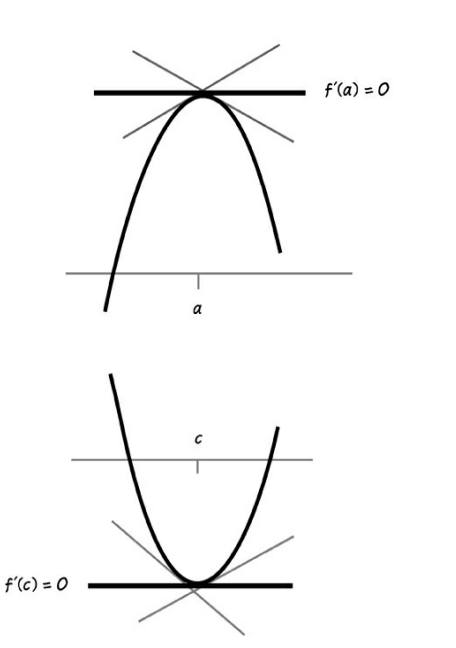
\includegraphics[width=0.75\linewidth]{Photos/Optimization zero slope.png}
    \caption{The turnings have become significant}
    
\end{figure}
We can notice that the slope of the tangent is $0$ at the points of maxima and minima. Hence, the extreme points are the roots of $f'(x)$.\\
But its not as simple, the converse is not always true, zero slope may just be a point of inflection(a point higher or lower than its neighbours but not the maxima or minima)\\
We need to be able to tell weather tell if a point is a maxima or a minima, so here is what we need to notice. The slope starts as positive for a maxima and then becomes negative. The opposite is true for minima. This means that we can take the rate of change of the slope and if it is less than $0$, the point is a maxima. If it is more than $0$, the point is a minima.\\
This is the second derivative test. But what if we don't wish to take two derivatives?\\
The we can notice that the sign of the slope changes at the points. So we can notice the value of $f'(x)$ between two roots to guess if its a minima or maxima.\\
We don't need to do this for every interval as the sign just alternates.\\
You'll understand this better through a problem:\\
\begin{example}
    An open topped box is to be constructed by removing equal squares from
each corner of a 3 metre by 8 metre rectangular sheet of aluminium and folding up the sides. Find the volume of the largest such box.
\end{example}
\begin{proof}
    [Solution]
    Let the side of the square removed be $x$. We can notice that the volume would be $f(x)=x(3-2x)(8-2x)=4x^3-22x^2+24x$  meter cubed.\\
    We can differentiate it to get the equation: $f'(x)=12x^2-44x+24$\\
    Setting this as zero has two solutions, $x=\frac{2}{3}, 3$\\
    While we know the answer is $\frac{2}{3}$ as one side of the shape is $3$. Let's confirm it is the maxima using both the methods.\\
    Single Derivative method: We can notice that $f'(0)=24>0$ which means that $f'(x)$ is positive till $x=\frac{2}{3}$, then negative till $x=2$, and then positive forever. \\
    We can use this to say $x=\frac{2}{3}$ is the point of maxima and $x=3$ the point of minima(realistically it is $x=\frac{3}{2}$)
Double derivative method: We can compute that $f''(x)=24x-44$ which is less than zero for $x=\frac{2}{3}$ and greater than zero for $x=3$ making them the maxima and minima repectivly.\\
With the tests out of the way, we can now find the largest possible volume by just plugging in $x=\frac{2}{3}$ to get that the maximum volume would be: $\frac{200}{3}$ meter cubed.
\end{proof}
And finally, we talk about video games. Most video games need to make trigonometric calculations in an instant especially online FPS and fighting games. While we could have it compute the actual values, that would be mind numbingly slow and make the gameplay worse. For the quick tactile feel we need, we use approximations. However, these approximations also need to be accurate or else the game will feel unrealistic.\\
How do we achieve this? Remember the mouse-flea discussion and its form we had created during the proof of L'-Hopital?\\
$f(x+h)=f(x)+hf'(x)$ may seem harmless enough but if we choose a value of $f(x)$ we already know and then move recursively ahead we can get increasingly accurate answers.\\
\begin{example}
    Calculate $\sqrt{73}$
\end{example}
\begin{proof}
    [Solution]
    Let's take $f(x)=\sqrt{x}$ and $x=8^2=64$,\\
    $\therefore h=73-64=9$ and $f'(x)=\frac{1}{2\sqrt{x}}$\\
Then we can say that, \\
$\sqrt{73}=f(73)=f(64+9)=f(64)+9f'(64)=8+\frac{9}{16}\\
= 8.5625$\\
The actual value of $\sqrt{73}=8.54400$ which is within $1\%$ of what we found using the formula only once.\\
A computer would now compute $8.5625^2$ and use that for an even more refined approximation. Most games do it 2-3 times, while even some calculators also use this but do it 5-10 times.\\
\end{proof}
And with that this chapter is concluded. 
\begin{xcb}{Exercises}
\begin{enumerate}
\item What is the co domain of $f(X)=\arctan(x)+\frac{1}{2}\arcsin(x)$?\\
\item Evaluate \[\lim_{x \to \frac{-1}{3}} \frac{1}{x} [\frac{-1}{x}]\] where $[x]$ represents the Greatest integer less than or equal to $x$
\item Evaluate: \[\lim_{n \to \infty} \frac{5^{n+1}+3^n-2^{2n}}{5^{n}+3^{2n+3}+2^{n}}\]
\item The value of the given limit is: \[\lim_{x \to 0} \frac{\cos(\sin(x))-\cos(x)}{x^4}\]
\item If \[\lim_{n \to \infty} \frac{1^2n+2^2(n-1)+3^2(n-2)+\dots+n^21}{1^3+2^3+^3+\dots +n^3} = \frac{a}{b}\] then find the value of $a^3+b^3$
\item \[\lim_{x \to 0} (\sum^n_{r=1} r^{\csc^2(x)})^{\sin^2(x)}\]
\item \[\lim_{n \to \infty} [(1+\frac{1}{n})^n-(1-\frac{1}{n})]^{-n}\]
\item  If $a_1$ is the greatest value of $f(x)$, where $f(x)=\frac{1}{2+[\sin(x)]}$ and $a_{n+1}=a_n+\frac{(-1)^{n+2}}{n+1}$, then $\lim_{n \to \infty} a_n =?$(here $[x]$ is the greatest integer function)\\
\item Calculate \[\lim_{x \to 0} \{[\frac{100x}{\sin(x)}] + [\frac{99 \sin(x)}{x}]\}\]
\item If $a_n$ and $b_n$ are positive integers and $a_n+\sqrt{2}b_n=(2+\sqrt{2})^n$ then calculate $\lim_{n \to \infty} (\frac{a_n}{b_n})=?$
\item If $f(x)=\begin{cases}
    k\sqrt{x+1}, \text{if} x\leq 3\\
    2+mx, \text{if} x> 3\\
\end{cases}$ is diffrentiatable at $x=3$, then find the vale if $m$ and $k$ is:
\item (JEE Mains 2018) Let $S = {t \in R:f(x)=|x -\pi|\cdot(e^{|x|} - 1)\sin(x) \text{is not differentiable at } t}$ then the set $S$ is equal to:
\item(JEE Mains 2021) The number of points at which the function $f(x)=|2x+1|-3|x+2|+|x^2+x-2|$ with $x \in \mathbb{R}$ is not differentiable, is: 
\item Let $f(x)=e^{x-1}-ax^2+b$ and $g(x)=\begin{cases}
    e^{x-1} \text{if} x \leq 1\\
    x^2+1 \text{if} x > 1\\
\end{cases}$ then find the value of $a$ and $b$ such that $f(x) \times g(x)$ is differentiable at $x=1$
\item (JEE Mains 2020) For a function $f$ defined on $(\frac{-1}{3},\frac{1}{3})$ by $f(x)= \begin{cases}
    \frac{1}{x} \ln{\frac{1+3x}{1-2x}} \text{ when } x \neq 0\\
    k, \text{ when } x=0
\end{cases}$ is continous, then $k$ is equal to\\
\item (AIEEE 2011) The value of $p$ and $q$ for which the function:\\
\[f(x)=\begin{cases}
    \frac{\sin(p+1)x+\sin(x)}{x}, x<0\\
    q, x=0\\
    \frac{\sqrt{x^2+x}-\sqrt{x}}{x^{\frac{3}{2}}}, x>0
\end{cases}\]
is continuous for all $x \in \mathbb{R}$ are
\item (JEE Mains 2020) If $y(a)=\sqrt{2(\frac{\tan(x)+\cot(x)}{1+\sin^2(a)}+\frac{1}{\sin^2(a)}}$ where $a \in (\frac{3\pi}{4}, \pi)$, then $\frac{dy}{dx}$ at $y=\frac{5\pi}{6}$ is:\\
\item(IIT 2006) If $f''(x)=-f(x)$ and $g(x)=f'(x)$ and $F(x)=(f(\frac{x}{2}))^2+(g(\frac{x}{2}))^2$ and given that $F(5)=5$, then $F(10)$ is
\item (IIT Adv 2014) Let $f : \mathbb{R} \to  \mathbb{R}$ and $g : \mathbb{R} \to  \mathbb{R}$ be respectively given by $f(x) = |x| + 1$ and $g(x) = x^2 + 1$. Defined $h:  \mathbb{R} \to  \mathbb{R}$ by $h(x)=\begin{cases}
    \max \{f(x),g(x)\}, x \leq 0\\
    \min \{f(x),g(x)\}, x > 0\\
\end{cases}$ The number of points at which $h(x)$ is not differentiable is:
\end{enumerate}
\end{xcb}